\documentclass[letterpaper]{article}
\usepackage[margin=1in]{geometry}
\usepackage[utf8]{inputenc}
\usepackage{textcomp}
\usepackage{amssymb}
\usepackage{natbib}
\usepackage{graphicx}
\usepackage{gensymb}
\usepackage{amsthm, amsmath, mathtools}
\usepackage[dvipsnames]{xcolor}
\usepackage{enumerate}
\usepackage{mdframed}
\usepackage[most]{tcolorbox}
\usepackage{csquotes}
% https://tex.stackexchange.com/questions/13506/how-to-continue-the-framed-text-box-on-multiple-pages

\tcbuselibrary{theorems}

\newcommand{\R}{\mathbb{R}}
\newcommand{\Z}{\mathbb{Z}}
\newcommand{\N}{\mathbb{N}}
\newcommand{\Q}{\mathbb{Q}}
\newcommand{\C}{\mathbb{C}}
\newcommand{\code}[1]{\texttt{#1}}
\newcommand{\mdiamond}{$\diamondsuit$}
\newcommand{\PowerSet}{\mathcal{P}}
\newcommand{\Mod}[1]{\ (\mathrm{mod}\ #1)}
\DeclareMathOperator{\lcm}{lcm}

%\newtheorem*{theorem}{Theorem}
%\newtheorem*{definition}{Definition}
%\newtheorem*{corollary}{Corollary}
%\newtheorem*{lemma}{Lemma}
\newtheorem*{proposition}{Proposition}


\newtcbtheorem[number within=section]{theorem}{Theorem}
{colback=green!5,colframe=green!35!black,fonttitle=\bfseries}{th}

\newtcbtheorem[number within=section]{definition}{Definition}
{colback=blue!5,colframe=blue!35!black,fonttitle=\bfseries}{def}

\newtcbtheorem[number within=section]{corollary}{Corollary}
{colback=yellow!5,colframe=yellow!35!black,fonttitle=\bfseries}{cor}

\newtcbtheorem[number within=section]{lemma}{Lemma}
{colback=red!5,colframe=red!35!black,fonttitle=\bfseries}{lem}

\newtcbtheorem[number within=section]{example}{Example}
{colback=white!5,colframe=white!35!black,fonttitle=\bfseries}{def}

\newtcbtheorem[number within=section]{note}{Important Note}{
        enhanced,
        sharp corners,
        attach boxed title to top left={
            xshift=-1mm,
            yshift=-5mm,
            yshifttext=-1mm
        },
        top=1.5em,
        colback=white,
        colframe=black,
        fonttitle=\bfseries,
        boxed title style={
            sharp corners,
            size=small,
            colback=red!75!black,
            colframe=red!75!black,
        } 
    }{impnote}
\usepackage[utf8]{inputenc}
\usepackage[english]{babel}
\usepackage{fancyhdr}
\usepackage[hidelinks]{hyperref}

\pagestyle{fancy}
\fancyhf{}
\rhead{Math 187A}
\chead{Wednesday, January 25, 2023}
\lhead{Lecture 5}
\rfoot{\thepage}

\setlength{\parindent}{0pt}

\begin{document}
\section{Classical Cryptosystems}
(Continued from previous lecture.)

\subsection{Interlude: Modular Linear Algebra}
Before going into polygraphic ciphers, let us first discuss how \emph{linear algebra} interacts with modular arithmetic. We'll just work on $2 \times 2$ matrices for now.

\subsubsection{\texorpdfstring{$2 \times 2$ Matrices}{2 by 2 Matrices}}

\begin{definition}{}{}
    A $2 \times 2$ integer \textbf{matrix} (or just \emph{matrix} for short) is a $2 \times 2$ box of numbers $A = \begin{bmatrix}
        a & b \\ c & d
    \end{bmatrix}$ where $a, b, c, d \in \Z$. 
    \begin{itemize}
        \item The \textbf{determinant} of $A$ is the integer $\det(A) = ad - bc$. 
        \item The \textbf{identity matrix} is the matrix $I = \begin{bmatrix}
            1 & 0 \\ 0 & 1
        \end{bmatrix}$. 
        \item Suppose $A = \begin{bmatrix}
            a & b \\ c & d
        \end{bmatrix}$ and $B = \begin{bmatrix}
            a' & b' \\ c' & d'
        \end{bmatrix}$ are two matrices. Their product $AB$ is defined to be \[AB = \begin{bmatrix}
            aa' + bc' & ba' + db' \\ ca' + dc' & cb' + dd'
        \end{bmatrix}.\]
    \end{itemize}
\end{definition}

\begin{mdframed}
    (Example.) Let $A = \begin{bmatrix}
        3 & 2 \\ 1 & 7
    \end{bmatrix}$ and $B = \begin{bmatrix}
        1 & 4 \\ 2 & 3
    \end{bmatrix}$. We know that \[\det(A) = 3 \cdot 7 - 2 \cdot 1 = 19.\] We also know that \[AB = \begin{bmatrix}
        7 & 18 \\ 15 & 25
    \end{bmatrix}\] and \[BA = \begin{bmatrix}
        7 & 30 \\ 9 & 25
    \end{bmatrix}.\] 
\end{mdframed}
\textbf{Remark:} It should be clear from the above example that $AB \neq BA$. That is, matrix multiplication is not commutative. 

\begin{mdframed}
    (Exercise.) Let $A$ be a $2 \times 2$ integer matrix. Show that \[AI = IA = A.\]

    \begin{mdframed}
        Let $A = \begin{bmatrix}
            a & b \\ 
            c & d
        \end{bmatrix}.$ Then, 
        \[IA = \begin{bmatrix}
            1 & 0 \\ 
            0 & 1
        \end{bmatrix} \begin{bmatrix}
            a & b \\ 
            c & d
        \end{bmatrix} = \begin{bmatrix}
            a & b \\ 
            c & d
        \end{bmatrix}\]
        and 
        \[AI = \begin{bmatrix}
            a & b \\ 
            c & d
        \end{bmatrix} \begin{bmatrix}
            1 & 0 \\ 
            0 & 1
        \end{bmatrix} = \begin{bmatrix}
            a & b \\ 
            c & d
        \end{bmatrix}.\]
    \end{mdframed}
\end{mdframed}

\begin{theorem}{Multiplicativity of Determinant}{}
    If $A$ and $B$ are matrices, then $\det(I) = 1$ and \[\det(AB) = \det(A)\det(B).\]
\end{theorem}

\begin{definition}{}{}
    A \textbf{vector} $v$ is a vertical column \[v = \begin{bmatrix}
        x \\ y
    \end{bmatrix},\] where $x, y \in \Z$. 
\end{definition}

\begin{definition}{}{}
    If $A = \begin{bmatrix}
        a & b \\ c & d
    \end{bmatrix}$ is a matrix, then the product $Ab = \begin{bmatrix}
        ax + by \\ 
        cx + dy
    \end{bmatrix}$.
\end{definition}

\subsubsection{Congruences and Inversion for Matrices}
\begin{definition}{}{}
    Fix a positive integer $n$ and suppose $A$ and $B$ are both matrices: 
    \[A = \begin{bmatrix}
        a & b \\ c & d
    \end{bmatrix}, \quad B = \begin{bmatrix}
        a' & b' \\ c' & d'
    \end{bmatrix}.\] We say that $A \equiv B \Mod{n}$ if all four of the entries of the two matrices are congruent mod $n$, i.e., if all of the following are true:  
    \[a \equiv a' \Mod{n}\] 
    \[b \equiv b' \Mod{n}\] 
    \[c \equiv c' \Mod{n}\]
    \[d \equiv d' \Mod{n}\]
\end{definition}

\begin{definition}{}{}
    A matrix $A$ is \emph{invertible mod} $n$ if there exists a matrix $X$ such that $AX \equiv I \Mod{n}$. In this case, $X$ is called an inverse of $A \Mod{n}$. In symbols, we write $X \equiv A^{-1} \Mod{n}$. 
\end{definition}

\begin{theorem}{Modular Inversion Theorem}{}
    Suppose $A = \begin{bmatrix}
        a & b \\ c & d
    \end{bmatrix}$ is a matrix. Then, $A$ is invertible if and only if $\det(A)$ is invertible mod $n$. Moreover, if $e \equiv \det(A)^{-1} \Mod{n}$, then \[X = \begin{bmatrix}
        ed & -eb \\ 
        -ec & ea
    \end{bmatrix}\] is an inverse of $A \Mod{n}$. 
\end{theorem}

\begin{mdframed}
    (Example.) Suppose we have $A = \begin{bmatrix}
        3 & 2 \\ 1 & 7
    \end{bmatrix}$. We know that $\det(A) = 19$ is invertible mod 26, so $A$ is also invertible mod 26. We have \[19^{-1} \equiv 11 \Mod{26},\] so the formula for the inverse from the Matrix Inversion Theorem tells us that \[A^{-1} \equiv \begin{bmatrix}
        11 \cdot 7 & -11 \cdot 2 \\ -11 \cdot 1 & 11 \cdot 3 
    \end{bmatrix} \equiv \begin{bmatrix}
        77 & -22 \\ -11 & 33
    \end{bmatrix} \equiv \begin{bmatrix}
        25 & 4 \\ 15 & 7
    \end{bmatrix} \Mod{26}.\] In other words, \[X = \begin{bmatrix}
        15 & 4 \\ 15 & 7
    \end{bmatrix}\] is an inverse of $A$ mod 26. It follows that $AX = I$. 
\end{mdframed}

\begin{mdframed}
    (Exercise.) Which of the following matrices is invertible mod 26? 
    \begin{enumerate}[(a)]
        \item $\begin{bmatrix}
            7 & 5 \\ 3 & 3 
        \end{bmatrix}$
        \item $\begin{bmatrix}
            8 & 1 \\ 3 & 2 
        \end{bmatrix}$
        \item $\begin{bmatrix}
            4 & 2 \\ 1 & 2 
        \end{bmatrix}$
        \item $\begin{bmatrix}
            4 & 3 \\ 1 & 2
        \end{bmatrix}$
    \end{enumerate}

    \begin{mdframed}
        The answer is \textbf{D}. By calculating the determinant of each matrix, we see that the GCD of the determinant of the matrix and 26 is 1 for only D. 
    \end{mdframed}
\end{mdframed}

\begin{mdframed}
    (Exercise.) As a follow-up to the previous exercise, what is the inverse of the invertible matrix? 

    \begin{mdframed}
        TODO 
    \end{mdframed}
\end{mdframed}

\subsection{Hill Cipher}
The \emph{Hill Cipher} is the first polygraphic cipher we'll talk about. We'll focus on the digraphic case, which replaces 2 letters of plaintext at a time. Our \textbf{key} for this cipher is a matrix that is invertible mod 26. 

\begin{mdframed}
    (Example.) Suppose we want to encrypt the message \textbf{\code{You have saved us all}}. Begin with the usual encoding process: 
    \begin{mdframed}
        \begin{verbatim}
 Y  O  U  H  A  V  E  S  A  V  E  D  U  S  A  L  L
24 14 20  7  0 21  4 18  0 21  4  3 20 18  0 11 11\end{verbatim}
    \end{mdframed} 
    (The numbers below the letters represent the ranking of each letter.) Let's suppose our key is \[A = \begin{bmatrix}
        3 & 2 \\ 1 & 7
    \end{bmatrix},\] which has determinant 19 and is thus invertible mod 26. It follows that $A$ is an invertible matrix mod 26, which can thus be used as a key. 

    \bigskip 

    For encrypting, the idea is to go through the list of numbers, replacing each pair of numbers with the result of multiplying that pair by the matrix $A \Mod{26}$. For example, for the pair 24 and 14, we can make a vector containing these numbers, \[v = \begin{bmatrix}
        24 \\ 14
    \end{bmatrix},\] and then compute \[Av = \begin{bmatrix}
        3 & 2 \\ 1 & 7
    \end{bmatrix} \begin{bmatrix}
        24 \\ 14
    \end{bmatrix} \Mod{26} = \begin{bmatrix}
        100 \\ 122
    \end{bmatrix} \Mod{26} = \begin{bmatrix}
        22 \\ 18
    \end{bmatrix}.\]
    So, we replace the numbers 24 and 14 with the numbers 22 and 18, respectively. In other words, the first two letters of the message will be replaced by \code{W} and \code{S}, respectively. 

    \bigskip 

    We can continue this process with the next pair of numbers (20, 7), and so on. Eventually, we'll reach the end. Note that, if you have an odd number of letters, you can add an additional random letter at the end (e.g., \code{Z}). With this in mind, the net result is the ciphertext
    \begin{mdframed}
\begin{verbatim}
WSWRQRWAQRSZSQWZFE\end{verbatim}
    \end{mdframed}

    As you might expect, to decrypt a message, we just need to multiply the pairs of numbers by the \emph{inverse} of $A$ mod 26.
\end{mdframed}

\begin{mdframed}
    (Exercise.) Use the matrix \[A = \begin{bmatrix}
        3 & -1 \\ 2 & 5
    \end{bmatrix}\] as the key for a Hill cipher. Encrypt the message \code{Go to Lake Lerna}.

    \begin{mdframed}
        First, we verify that this matrix can be used as a key by checking the determinant.
        \[\det(A) = 15 - 2(-1) = 15 + 2 = 17.\]
        Because 17 is invertible mod 26, it follows that we can use $A$ as a key. So, begin by encoding the message: 
        \begin{mdframed}
            \begin{verbatim}
G  O  T  O  L A  K E  L E  R  N A  Z
6 14 19 14 11 0 10 4 11 4 17 13 0 25\end{verbatim}
        \end{mdframed}
        Note that we put a \code{Z} at the end so that the length of the plaintext is even (that way, we can do pairwise encryption.) We'll now process each pair of letters. 
        \begin{itemize}
            \item For pair $(6, 14)$, we have 
            \[\begin{bmatrix}
                3 & -1 \\ 2 & 5
            \end{bmatrix} \begin{bmatrix}
                6 \\ 14
            \end{bmatrix} \Mod{26} = \begin{bmatrix}
                4 \\ 82 
            \end{bmatrix} \Mod{26} = \begin{bmatrix}
                4 \\ 4
            \end{bmatrix},\]
            which corrsponds to \code{E} and \code{E}.

            \item For pair $(19, 14)$, we have 
            \[\begin{bmatrix}
                3 & -1 \\ 2 & 5
            \end{bmatrix} \begin{bmatrix}
                19 \\ 14
            \end{bmatrix} \Mod{26} = \begin{bmatrix}
                43 \\ 108
            \end{bmatrix} \Mod{26} = \begin{bmatrix}
                17 \\ 4
            \end{bmatrix} \Mod{26},\]
            which corresponds to \code{R} and \code{E}.

            \item For pair $(11, 0)$, we have 
            \[\begin{bmatrix}
                3 & -1 \\ 2 & 5
            \end{bmatrix} \begin{bmatrix}
                11 \\ 0
            \end{bmatrix} \Mod{26} = \begin{bmatrix}
                33 \\ 22
            \end{bmatrix} \Mod{26} = \begin{bmatrix}
                7 \\ 22
            \end{bmatrix} \Mod{26},\]
            corresponding to \code{H} and \code{W}.
        \end{itemize}
        By continuing this process, we end up with the ciphertext 
        \begin{mdframed}
\begin{verbatim}
EEREHWAODQMVBV\end{verbatim}
        \end{mdframed}
    \end{mdframed}
\end{mdframed}

\begin{mdframed}
    (Exercise.) Use the matrix \[A = \begin{bmatrix}
        3 & -1 \\ 2 & 5
    \end{bmatrix}\] as the key for a Hill cipher. Decrypt the message \code{RNCQYVFRRLZI}.

    \begin{mdframed}
        Note again that $\det(A) = 17$. In order to decrypt the message, we need to find the inverse of $A$ mod 26.

        \bigskip 

        \textbf{Finding GCD:} Recall that the Matrix Inversion Theorem states that $A$ is invertible if and only if $\det(A)$ is invertible mod $n$. To see if $\det(A)$ is invertible mod $n$, we need to see if $\gcd(\det(A), n) = 1$. So, let's find $\gcd(17, 26)$.  
        \begin{center}
            \begin{tabular}{c|c|c|c|c}
                $a$ & $b$ & $b = aq + r$ & $q$ & $r$ \\ 
                \hline 
                17 & 26 & $26 = 17q + r$ & 1 & 9 \\ 
                9 & 17 & $17 = 9q + r$ & 1 & 8 \\ 
                8 & 9 & $9 = 8q + r$ & 1 & 1 \\ 
                1 & 8 & $8 = 1q + r$ & 8 & 0
            \end{tabular}
        \end{center}
        Therefore, $\gcd(17, 26) = 1$ as desired. Thus, an inverse must exist. 

        \bigskip 
        
        \textbf{Finding Bezout:} Now, we need to find the Bezout coefficients. Labeling each equation, we have 
        \begin{itemize}
            \item (Eq. 1) $26 = 17(1) + 9 \implies 9 = 26 + 17(-1)$ 
            \item (Eq. 2) $17 = 9(1) + 8 \implies 8 = 17 + 9(-1)$
            \item (Eq. 3) $9 = 8(1) + 1 \implies 1 = 9 + 8(-1)$ 
        \end{itemize}
        Now that we've labeled each relevant operation, we can find the Bezout coefficients: 
        \begin{equation*}
            \begin{aligned}
                1 &= 9 + 8(-1) \\ 
                    &= 9 + (\underbrace{17 + 9(-1)}_{\text{Eq. 2}})(-1) \\ 
                    &= 9 + 17(-1) + 9(-1)(-1) \\ 
                    &= 9 + 17(-1) + 9 \\ 
                    &= 9(2) + 17(-1) \\ 
                    &= (\underbrace{26 + 17(-1)}_{\text{Eq. 1}})(2) + 17(-1) \\ 
                    &= 26(2) + 17(-1)(2) + 17(-1) \\ 
                    &= 26(2) + 17(-2) + 17(-1) \\ 
                    &= 26(2) + 17(-3)
            \end{aligned}
        \end{equation*}
        From this, it follows that $x = -3$, which is the desired inverse.  

        \bigskip 

        \textbf{Decrypting:} With this in mind, we have 
        \[X = \begin{bmatrix}
            -3(5) & 3(-1) \\ 3(2) & -3(3)
        \end{bmatrix} = \begin{bmatrix}
            -15 & -3 \\ 6 & -9
        \end{bmatrix} \Mod{26}.\]
        Now that we have the matrix needed to decrypt the message, we can proceed. Labeling each character in the message gives us 
        \begin{mdframed}
            \begin{verbatim}
R  N C  Q  Y  V F  R  R  L  Z I
17 13 2 16 24 21 5 17 17 11 25 8\end{verbatim}
        \end{mdframed}
    \end{mdframed}

    % a pretty stupid hack but at least the frames are readable like this
    \begin{mdframed}
        Iterating over each pair, we have 
        \begin{itemize}
            \item For $(17, 13)$, 
            \[X\begin{bmatrix}
                17 \\ 13
            \end{bmatrix} \Mod{26} = \begin{bmatrix}
                -294 \\ -15
            \end{bmatrix} \Mod{26} = \begin{bmatrix}
                18 \\ 11
            \end{bmatrix} \Mod{26},\]
            or \code{S} and \code{L}. 

            \item For $(2, 16)$, 
            \[X\begin{bmatrix}
                2 \\ 16
            \end{bmatrix} \Mod{26} = \begin{bmatrix}
                -78 \\ -132
            \end{bmatrix} \Mod{26} = \begin{bmatrix}
                0 \\ 24
            \end{bmatrix} \Mod{26},\]
            or \code{A} and \code{Y}.
        \end{itemize}
        By continuing this process, we end up with 
        \begin{mdframed}
            \begin{verbatim}
SLAYTHEHYDRA\end{verbatim}
        \end{mdframed}
    \end{mdframed}
\end{mdframed}

\begin{mdframed}
    (Exercise.) Use the Hill cipher with key \[A = \begin{bmatrix}
        4 & 3 \\ 1 & 2
    \end{bmatrix}\] to encrypt the word \code{AREA}. 

    \begin{mdframed}
        Labeling each letter with its corresponding number, we have 
        \begin{mdframed}
            \begin{verbatim}
0 17 4 0
A  R E A\end{verbatim}
        \end{mdframed}
        Then, we just need to multiply each pair of numbers, like so: 
        \[\begin{bmatrix}
            4 & 3 \\ 1 & 2
        \end{bmatrix} \begin{bmatrix}
            0 \\ 17
        \end{bmatrix} = \begin{bmatrix}
            4 \cdot 0 + 3 \cdot 17 \\ 
            1 \cdot 0 + 2 \cdot 17
        \end{bmatrix} = \begin{bmatrix}
            51 \\ 
            34 
        \end{bmatrix} \equiv \begin{bmatrix}
            25 \\ 
            8
        \end{bmatrix} \Mod{26},\]
        and 
        \[\begin{bmatrix}
            4 & 3 \\ 1 & 2 
        \end{bmatrix} \begin{bmatrix}
            4 \\ 0
        \end{bmatrix} = \begin{bmatrix}
            16 + 0 \\ 
            4 + 0
        \end{bmatrix} \equiv \begin{bmatrix}
            16 \\ 4
        \end{bmatrix} \Mod{26}.\] Therefore, the answer is \code{ZIQE}.
    \end{mdframed}
\end{mdframed}

\begin{mdframed}
    (Exercise.) The matrix \[A = \begin{bmatrix}
        4 & 3 \\ 1 & 2
    \end{bmatrix}\] is used to encrypt \code{CRZX}. What is the plaintext? 

    \begin{mdframed}
        We know that the inverse of $A$ is \[X =  \begin{bmatrix}
            16 & 15 \\ 
            5 & 6 
        \end{bmatrix}.\] Then, going through each pair of numbers gives us 
        \[\begin{bmatrix}
            16 & 15 \\ 5 & 6
        \end{bmatrix} \begin{bmatrix}
            2 \\ 17
        \end{bmatrix} = \begin{bmatrix}
            16 \cdot 2 + 15 \cdot 17 \\ 
            5 \cdot 2 + 6 \cdot 17
        \end{bmatrix} = \begin{bmatrix}
            287 \\ 
            112
        \end{bmatrix} = \begin{bmatrix}
            1 \\ 
            8
        \end{bmatrix},\]
        and 
        \[\begin{bmatrix}
            16 & 15 \\ 5 & 6
        \end{bmatrix} \begin{bmatrix}
            25 \\ 23
        \end{bmatrix} = \begin{bmatrix}
            16 \cdot 25 + 15 \cdot 23 \\ 
            5 \cdot 25 + 6 \cdot 23 
        \end{bmatrix} = \begin{bmatrix}
            745 \\ 263
        \end{bmatrix} \equiv \begin{bmatrix}
            17 \\ 3
        \end{bmatrix}.\]
        This gives us \code{BIRD}.
    \end{mdframed}
\end{mdframed}

\begin{mdframed}
    (Exercise.) Suppose you want to encrypt a sequence of bits (i.e., a sequence of \code{0}'s and \code{1}'s) using a $2 \times 2$ Hill cipher. How many different encryption functions are there? In other words, how many different congruence classes of $2 \times 2$ can be used as a key for a Hill cipher? 

    \begin{mdframed}
        If we assume that our alphabet contains only binary numbers, then there are 2 possible numbers. Therefore, our Hill cipher must be a matrix mod 2. We want to know how many of these matrices are invertible mod 2. 

        \bigskip 

        There are $2 \cdot 2 \cdot 2 \cdot 2$ choices for what our $2 \times 2$ matrix can be. There are three possible determinants: $0$ and $\pm 1$. Note that $-1 \equiv 1 \Mod{2}$ so there's actually \emph{2} possible determinants. Of these determinants, note that $\gcd(1, 2) = 1$ while $\gcd(0, 2) = 2$.
        
        \bigskip 

        With this in mind, we know that any matrix with determinant 1 is valid. There are \boxed{6} such matrices.
    \end{mdframed}
\end{mdframed}

\subsection{Playfair Cipher}
The \textbf{Playfair Cipher} is another digraphic cipher, like the Hill cipher we just discussed above. The key for a Playfair cipher is a $5 \times 5$ grid of letters, where each letter appears exactly once. Because there are 26 letters in the English alphabet but 25 letters can fit in a grid, we treat \code{I} and \code{J} as the same letter\footnote{We could also use a variant where we use a $6 \times 6$ grid that includes all 26 letters and 10 digits, instead.}. 

\bigskip 

How do we start constructing a grid? An easy and convenient way of doing this is to start with a secret keyword. For example, suppose \code{ALPHABET} is our keyword. We can start filling out our grid by writing out the letters of our keyword across the rows, skipping over the letters we've written.
\begin{center}
    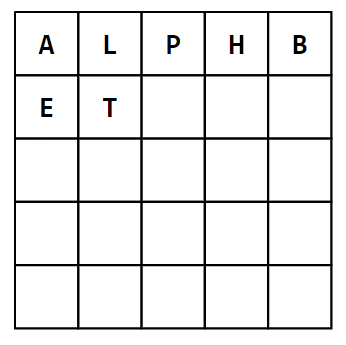
\includegraphics[scale=0.5]{../assets/playfair_1.png}
\end{center}
We can then fill out the remaining squares with the remaining letters of the alphabet, skipping over anything we've already written down and remembering that \code{I} and \code{J} are the same. 
\begin{center}
    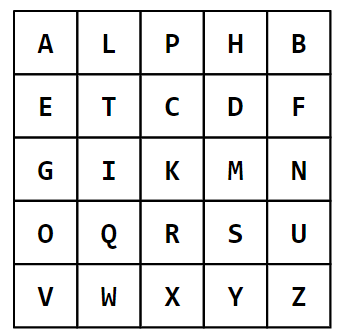
\includegraphics[scale=0.5]{../assets/playfair_2.png}
\end{center}
We can encode our message by doing the following: 
\begin{enumerate}
    \item Remove all non-alphabet characters and capitalize everything.
    \item Replace all instances of \code{J} with \code{I}. 
    \item Group the letters into pairs. 
    \item If there are any pairs where both letters are the same, inser the letter \code{X} in between the two letters of that pair and regroup into pairs. 
    \item If there's an unpaired letter at the end, insert the letter \code{X} after it.
\end{enumerate}
\textbf{Remark:} You may need to apply rule 4 multiple times. 

\begin{mdframed}
    (Example.) Suppose we want to encode the message \code{hidden jewels in trees.} Here's what will happen after each step described above. 
    \begin{enumerate}
        \item \code{HIDDENJEWELSINTHETREES}
        \item \code{HIDDENIEWELSINTHETREES}
        \item \code{HI DD EN IE WE LS IN TH ET RE ES}
        \item \code{HI DX DE NI EW EL SI NT HE TR EX ES}
        \item \code{HI DX DE NI EW EL SI NT HE TR EX ES}
    \end{enumerate}
\end{mdframed}

To encrypt, we need to replace each pair with another pair using the grid by following the rules: 
\begin{itemize}
    \item (Row Rule.) If both letters in the pair occur in the same row, replace each letter of the pair with the letter that appears immediately to its right (wrapping around to the left side of the row if needed).
    \item (Column Rule.) If both letters in the pair occur in the same column, replace each letter of the pair with the letter that appears immediately below it (wrapping around to the top of the column if needed).
    \item (Rectangle Rule.) Otherwise, the two letters define a rectangle inside the grid, and we replace each letter with the letter on the same row but the opposite of that rectangle.
\end{itemize}

\begin{mdframed}
    (Example.) Suppose we want to encrypt the message \code{HI DX DE NI EW EL SI NT HE TR EX ES} (see previous example for encoding). Let's look at each pair. 
    \begin{itemize}
        \item For \code{HI}, notice that \code{H} and \code{I} do not appear in the same row or column. Therefore, the rectangle rule applies. Observe the highlighted cells: 
        \begin{center}
            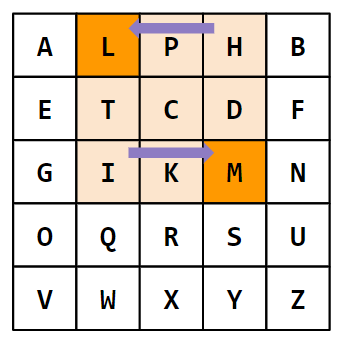
\includegraphics[scale=0.5]{../assets/playfair_3.png}
        \end{center}
        Here, the letter in the same row as \code{H} but opposite side is \code{L}, and the letter in the same row as \code{I} but the opposite side is \code{M}. Therefore, \code{HI} becomes \code{LM}. 


        \item For \code{DX}, we also apply the rectangle rule. Observe the highlighted cells: 
        \begin{center}
            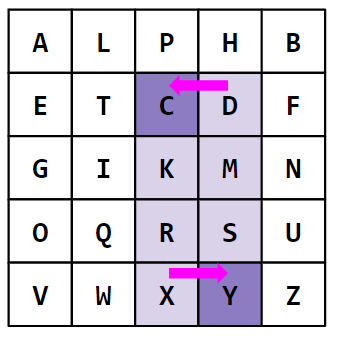
\includegraphics[scale=0.5]{../assets/playfair_4.png}
        \end{center}
        So, it follows that \code{DX} gets replaced with \code{CY}.

        \item For \code{DE}, both letters are on the same row so we apply the row rule. Observe that 
        \begin{center}
            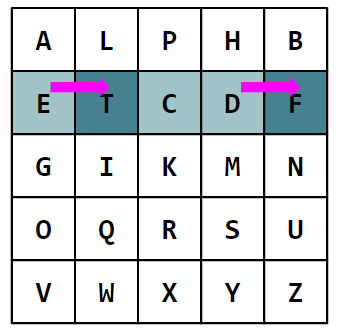
\includegraphics[scale=0.5]{../assets/playfair_5.png}
        \end{center}
        So, it follows that \code{DE} becomes \code{FT}.
    \end{itemize}
    Continuing this process yields the desired result.
\end{mdframed}

\begin{mdframed}
    (Exercise.) You are constructing a $5 \times 5$ grid for a Playfair cipher starting with the keyword \code{FAJITAS}. What letter falls in the very center of the grid (i.e., in the 3rd row and the 3rd column)? 

    \begin{enumerate}[(a)]
        \item K
        \item L
        \item M
        \item None of the above. 
    \end{enumerate}

    \begin{mdframed}
        Constructing the grid looks something like: 
        \begin{center}
            \begin{tabular}{|c|c|c|c|c|}
                \hline 
                F & A & I & T & S \\
                \hline 
                B & C & D & E & G \\
                \hline 
                H & K & L & M & N \\
                \hline 
                O & P & Q & R & U \\
                \hline 
                V & W & X & Y & Z \\ 
                \hline 
            \end{tabular}
        \end{center}
        So, the answer is (b). 
    \end{mdframed}
\end{mdframed}

\begin{mdframed}
    (Exercise.) Encode the message \code{Little Fluffy} for encryption using a Playfair cipher. How many pairs of letters are in the encoded message? 

    \begin{enumerate}[(a)]
        \item 6
        \item 7
        \item 8
        \item None of the above. 
    \end{enumerate}

    \begin{mdframed}
        Encoding gives us 
        \begin{itemize}
            \item LITTLEFLUFFY
            \item LITTLEFLUFFY
            \item LITXTLEFLUFXFY
            \item LI TX TL EF LU FX FY
        \end{itemize}
        The answer is (b). 
    \end{mdframed}
\end{mdframed}

\begin{mdframed}
    (Exercise.) Use a Playfair cipher with a key given by the grid below, decrypt \code{WZ LT OP WK SH ES VX PH}.
    \begin{center}
        \begin{tabular}{|c|c|c|c|c|}
            \hline
            C & W & F & Q & Y \\ 
            \hline
            G & I & Z & R & B \\ 
            \hline
            H & M & K & L & U \\ 
            \hline
            V & A & D & E & N \\ 
            \hline
            O & P & X & T & S \\ 
            \hline
        \end{tabular}
    \end{center}

    \begin{mdframed}
        For decryption, we just perform the inverse of the encryption process (e.g., for the row rule, when encrypting is replacing the letter with the one immediately to the right, decrypting is replacing the letter with the one immediately to the left.)
        \begin{itemize}
            \item \code{WZ} maps to \code{FI}.
            \item \code{LT} maps to \code{RE}.
            \item \code{OP} maps to \code{SO}.
            \item \code{WK} maps to \code{FM}.
            \item \code{SH} maps to \code{OU}.
            \item \code{ES} maps to \code{NT}.
            \item \code{VX} maps to \code{DO}.
            \item \code{PH} maps to \code{OM}.
        \end{itemize}
        The answer is \code{FIRESOFMOUNTDOOM}, or \code{Fires of Mount Doom}.
    \end{mdframed}
\end{mdframed}


\end{document}